\documentclass[aps,prd,twocolumn,superscriptaddress,nofootinbib,floatfix]{revtex4-2}

\usepackage{amsmath,amssymb,amsfonts}
\usepackage{graphicx}
\usepackage{booktabs}
\usepackage{hyperref}
\usepackage{cleveref}
\crefname{paragraph}{Section}{Sections}
\Crefname{paragraph}{Section}{Sections}
\usepackage{xcolor}
\usepackage{bm}
\usepackage{enumitem}

% math_commands.tex — shared notation for DSC CMB paper
\newcommand{\R}{\mathbb{R}}
\newcommand{\Z}{\mathbb{Z}}
\newcommand{\N}{\mathbb{N}}
\newcommand{\calL}{\mathcal{L}}
\newcommand{\calM}{\mathcal{M}}

% DSC-specific
\newcommand{\lnln}{\ln^2}
\newcommand{\ac}{a_c}
\newcommand{\kopt}{k_{\mathrm{opt}}}
\newcommand{\mudyn}{\mu_{\mathrm{dyna}}}
\newcommand{\ceff}{c^2_{\mathrm{eff}}}
\newcommand{\Hinfty}{H_\infty}
\newcommand{\tP}{t_{\mathrm{P}}}
\newcommand{\lP}{\ell_{\mathrm{P}}}
\newcommand{\nside}{N_{\mathrm{side}}}

% Operators
\DeclareMathOperator*{\argmin}{arg\,min}
\DeclareMathOperator{\Tr}{Tr}


\graphicspath{{../figures/}}

\begin{document}

\title{Differentiable Discrete Symplectic Cosmology: Cross-Scale Empirical Tests of a $1/\ln^2(t)$ Cooling Law}

\author{Liang Wang}
\email{wangliang.f@gmail.com}
\affiliation{School of Artificial Intelligence and Automation, Huazhong University of Science and Technology, 430070, P.R. China}

\begin{abstract}
We explore whether the Discrete Symplectic Cosmology (DSC) framework---in which cosmic evolution is modeled as a non-autonomous symplectic map on a Planck-scale lattice with a $1/\ln^2(t)$ adiabatic cooling law motivated by Riemann zero spectral statistics---can reproduce key statistical features of the cosmic microwave background (CMB) temperature anisotropies.
Using a St\"ormer--Verlet integrator on two- and three-dimensional lattices, we find that: (i) the symplectic evolution produces near-Gaussian one-point statistics (skewness $= +0.07 \pm 0.30$, excess kurtosis $= -0.28 \pm 0.24$ over 20 independent realizations), while a dissipative coupled-map-lattice baseline fails with kurtosis $= -1.60$; (ii) acoustic-like oscillation peaks emerge in the power spectrum $D(k) = k^2 P(k)$, with positions alignable to a toy analytic reference via three lattice parameters; (iii) the $1/\ln^2(t)$ cooling produces an effective acoustic freeze-out through asymptotic deceleration of wave propagation; and (iv) Bayesian optimization recovers all three lattice parameters from power spectra in a twin experiment (MSE $= 8.9 \times 10^{-5}$).
Full-sky maps generated by projecting a $128^3$ lattice onto a HEALPix sphere exhibit multi-scale temperature fluctuations with pixel distributions close to those of the Planck SMICA map, though quantitative comparison of the angular power spectrum yields $\chi^2/\mathrm{dof} \approx 3.3$, indicating that the forward model does not yet reproduce the observed $C_\ell$ at the level of individual multipoles.
A differentiable implementation in JAX enables gradient-based inverse reconstruction from Planck data (pixel correlation $r = 0.98$), but a held-out hemisphere test ($r = -0.17$) confirms that the severely underdetermined inverse problem does not uniquely constrain the 3D structure.
These results establish the DSC lattice as an exploratory proof-of-concept framework for generating CMB-like fluctuations from symplectic dynamics, while highlighting the substantial gap between phenomenological similarity and quantitative agreement with the observed CMB.
\end{abstract}


\maketitle

\section{Introduction}
\label{sec:intro}

The temperature anisotropies of the cosmic microwave background (CMB), as mapped by the Planck satellite~\citep{Planck2018VI}, encode a remarkably simple statistical portrait of the early universe: the fluctuations are nearly Gaussian, their angular power spectrum exhibits a series of acoustic peaks at multipoles $\ell \sim 220, 540, 810, \ldots$, and the comoving sound horizon at recombination is finite.
In the standard $\Lambda$CDM paradigm, these features arise from quantum fluctuations amplified by inflation and processed by the baryon--photon plasma prior to decoupling.

Recently, a phenomenological framework called \emph{Discrete Symplectic Cosmology} (DSC) was proposed~\citep{Wang2026}, in which cosmic evolution is modeled as a non-autonomous dynamical system on a Planck-scale lattice $\Z^3 \times \N$.
Three structural assumptions---discrete spacetime, symplectic evolution, and a Berry--Keating spectral correspondence---motivate an adiabatic cooling law of the form
\begin{equation}
  \mu(n) = \mudyn + \frac{\kopt}{\ln^2(n + c_0)}\,,
  \label{eq:cooling}
\end{equation}
where $n$ is the discrete Planck time, $\mudyn$ is the asymptotic critical value, $\kopt$ is related to Feigenbaum scaling, and $c_0$ regularizes small $n$.
This $1/\ln^2$ functional form is slower than any power law and is singled out by the Riemann zero spectral density~\citep{Wang2026}.
The framework yields a dynamical cosmological term $\Lambda(t) = \Lambda_\infty + \gamma / \ln^2(t/\tP)$ and a Hubble relaxation law $H(t) = \Hinfty + \beta / \ln^2(t/\tP)$, providing a candidate mechanism for modifying the early expansion rate without introducing new scalar fields.

However, the original DSC work validates the cooling law only through one-dimensional H\'enon map surrogates.
The question of whether spatially-extended lattice dynamics---evolving under the DSC cooling law---can reproduce the \emph{spatial} statistical features of the CMB remains open.
We stress that the present work is \emph{exploratory}: the lattice simulations are effective surrogate models, not direct implementations of Planck-scale quantum gravity.
The goal is to investigate what phenomenological features emerge from the DSC dynamical assumptions, not to claim a complete alternative to $\Lambda$CDM.
In particular: does a symplectic lattice produce Gaussian fluctuations?
Do acoustic oscillation peaks emerge?
Is the acoustic horizon finite?

In this paper, we address these questions by implementing St\"ormer--Verlet symplectic integrators on two- and three-dimensional lattices with DSC-motivated cooling.
Our main findings are:

\begin{enumerate}
  \item \textbf{Near-Gaussian one-point statistics.}
  Symplectic lattice evolution produces temperature fluctuations with skewness $\approx +0.07$ and excess kurtosis $\approx -0.28$ (ensemble of 20 runs), consistent with Gaussianity.
  An ablation study shows that a dissipative coupled-map-lattice (CML) baseline produces kurtosis $= -1.60$ and fails to match $\Lambda$CDM spectral shape (Pearson $r = 0.74$ vs.\ $r = 0.96$ for the symplectic model).

  \item \textbf{Acoustic-like oscillation peaks.}
  The scaled power spectrum $D(k) = k^2 P(k)$ exhibits 5--6 peaks from pure symplectic wave propagation.
  A three-parameter phenomenological fit aligns all peak positions to a mock $\Lambda$CDM reference (MSE $= 8.9 \times 10^{-5}$).

  \item \textbf{Finite acoustic horizon via freeze-out.}
  The $1/\ln^2(t)$ decay of the effective sound speed causes wavefronts to asymptotically freeze, producing a finite comoving horizon $r_s \approx 38$ lattice units without requiring abrupt decoupling.

  \item \textbf{Parameter recovery via simulation-based inference.}
  A Bayesian optimization twin experiment recovers all three lattice parameters ($c^2$, drag, $\kopt$) from the power spectrum.

  \item \textbf{Planck-comparable full-sky maps.}
  Three-dimensional lattice evolution projected onto a HEALPix sphere produces CMB-like full-sky maps with pixel distributions close to the Planck SMICA map (skewness $-0.075 \pm 0.009$ vs.\ Planck $-0.036$).

  \item \textbf{Differentiable inverse reconstruction.}
  The DSC physics engine is fully differentiable: gradient-based optimization recovers the 3D primordial field from Planck sky data with pixel correlation $r = 0.98$.
  While naive 2D-only optimization hits the fundamental line-of-sight degeneracy ($r < 0$ on held-out hemisphere), we show that sparse volumetric priors (mock 3D survey anchors) partially break this degeneracy, and the reconstructed 3D field spontaneously obeys the $P(k) \propto k^{-3}$ gravity scaling.

  \item \textbf{Full cosmic timeline with V-shape transition.}
  Evolving the reconstructed initial conditions beyond the CMB epoch with nonlinear gravitational terms reveals a V-shape thermodynamic transition: the $1/\ln^2(t)$ cooling naturally smooths primordial chaos (decreasing field variance), while subsequent Jeans instability rebuilds structural complexity into a cosmic web---providing a smoothing mechanism analogous to inflation without an ad-hoc scalar field.
\end{enumerate}

The remainder of this paper is organized as follows.
\Cref{sec:background} summarizes the DSC theoretical framework.
\Cref{sec:methods} describes the numerical methods.
\Cref{sec:results} presents the simulation results.
\Cref{sec:discussion} discusses the physical interpretation and relation to standard cosmology.
\Cref{sec:limitations} lists limitations, and \Cref{sec:conclusion} concludes.

\section{Theoretical Background}
\label{sec:background}

\subsection{The DSC framework}
\label{sec:dsc}

Discrete Symplectic Cosmology (DSC)~\citep{Wang2026} models cosmic evolution as a non-autonomous dynamical system on a four-dimensional lattice $\calL = \Z^3 \times \N$, where spatial sites are separated by the Planck length $\lP = \sqrt{\hbar G/c^3} \approx 1.616 \times 10^{-35}$\,m and temporal ticks by the Planck time $\tP = \sqrt{\hbar G/c^5} \approx 5.391 \times 10^{-44}$\,s.
Three assumptions define the framework:

\paragraph{Assumption 1 (Discrete spacetime).}
Spacetime is a cubic lattice at the Planck scale.  Each site $(\bm{x}, n) \in \Z^3 \times \N$ carries a local state $\phi_n(\bm{x}) \in \calM$, where $\calM$ is a finite-dimensional phase-space manifold.

\paragraph{Assumption 2 (Symplectic evolution).}
The one-step evolution map $F_n : \Phi_n \mapsto \Phi_{n+1}$ is a symplectomorphism with respect to a discrete symplectic 2-form $\omega$:
\begin{equation}
  F_n^* \omega = \omega \quad \forall\, n\,.
  \label{eq:symp}
\end{equation}
Concretely, this requires $\det DF_n = 1$ (Liouville's theorem on the lattice), ensuring three properties: (i) unitarity---phase-space volume is preserved; (ii) reversibility---$F_n$ is invertible, consistent with CPT symmetry; and (iii) energy-error boundedness---by the backward error analysis of symplectic integrators~\citep{Hairer2006}, $F_n$ is the \emph{exact} flow of a nearby Hamiltonian, preventing secular energy drift over cosmological timescales.

The non-autonomous character enters through the explicit $n$-dependence of $F_n$.  Following the theory of non-autonomous dynamical systems~\citep{Kloeden2011}, the sequence $\{F_n\}_{n \in \N}$ is viewed as a process (or two-parameter semigroup) and studied via its pullback attractors.

\paragraph{Assumption 3 ($1/\ln$ spectral density of the lattice Hamiltonian).}
We posit that the spectral density of the (effective) lattice Hamiltonian satisfies a logarithmic counting law of the Riemann--von Mangoldt form,
\begin{equation}
  \rho(E) = \frac{1}{2\pi}\ln\!\left(\frac{E}{2\pi}\right) + O\!\left(\frac{1}{E}\right)\,,
  \label{eq:rvm}
\end{equation}
which is mathematically the same form satisfied by the Riemann zeta zeros.
This is an \emph{ansatz} on the spectral density, not a derivation: we adopt it because it produces a closed-form $1/\ln^2$ cooling law (\cref{sec:cooling_derivation}) that is the central testable hypothesis of this paper.
We do not engage with the broader question of whether a physical Hamiltonian exists whose eigenvalues are literally the Riemann zeros (the Hilbert--P\'olya program), nor with experimental programs aimed at realizing such a spectrum in laboratory systems.
The numerical spectral observation that period-doubling renormalization flow exhibits a level-counting law of the same logarithmic form~\citep{Wang2026} provides additional motivation for adopting \cref{eq:rvm} as the working ansatz.

\subsection{Derivation of the $1/\ln^2$ cooling law}
\label{sec:cooling_derivation}

The $1/\ln^2$ functional form is not arbitrary; it follows from the spectral density \cref{eq:rvm}.
The mean level spacing of the quantized lattice Hamiltonian is
\begin{equation}
  \Delta E(n) \sim \frac{1}{\rho(n)} \sim \frac{2\pi}{\ln(n)}\,,
  \label{eq:spacing}
\end{equation}
where $n = t/\tP$ is the Planck tick number.
The residual vacuum energy fluctuation---identified with the variance of the zero-point energy around the ground state---scales as the square of the level spacing:
\begin{equation}
  \delta\rho_{\mathrm{vac}}(n) \propto (\Delta E)^2 \sim \frac{1}{\ln^2(n)}\,.
  \label{eq:vac}
\end{equation}
Identifying this fluctuation with the time-dependent part of the control parameter yields
\begin{equation}
  \mu(n) = \mudyn + \frac{\kopt}{\ln^2(n + c_0)}\,,
  \label{eq:cooling_full}
\end{equation}
where $\mudyn \approx 1.5437$ is the asymptotic critical value (the 2D effective critical baseline), $\kopt \approx \alpha_F/2 \approx 1.248$ is conjectured to relate to the Feigenbaum spatial rescaling constant $\alpha_F = 2.5029\ldots$, and $c_0 = 10$ regularizes the logarithmic divergence at $n = 0$.

This is the \emph{physically motivated} cooling schedule: $p = 2$ is singled out among the family $\epsilon(n) = k/\ln^p(n)$ as the unique exponent for which (a) the time-averaged Lyapunov exponent $\bar{\lambda}(N) \to 0$ as $N \to \infty$ (asymptotic criticality), and (b) the cumulative perturbation $\sum \sqrt{\epsilon(n)}$ diverges (non-trivial exploration), while (c) the Riemann zero density provides the physical value $p = 2$~\citep{Wang2026}.

The framework yields two key cosmological consequences:
\begin{itemize}
  \item A dynamical cosmological term~\citep{Wang2026}:
  \begin{equation}
    \Lambda(t) = \Lambda_\infty + \frac{\gamma}{\ln^2(t/\tP)}\,,
    \label{eq:lambda}
  \end{equation}
  entering the Friedmann equation as a time-dependent vacuum energy density.
  \item A Hubble relaxation law:
  \begin{equation}
    H(t) = \Hinfty + \frac{\beta}{\ln^2(t/\tP)}\,,
    \label{eq:hubble}
  \end{equation}
  predicting monotone relaxation toward an asymptotic rate $\Hinfty = \sqrt{\Lambda_\infty/3} < H_0$.
\end{itemize}

\subsection{From H\'enon maps to St\"ormer--Verlet}
\label{sec:sv}

The original DSC paper validates the cooling law using the area-preserving H\'enon map ($b = -1$, $\det DF = 1$) as a one-dimensional surrogate.
In the present work, we extend to spatially coupled $d$-dimensional lattices ($d = 2, 3$) using the St\"ormer--Verlet symplectic integrator:
\begin{equation}
  \phi_{n+1} = 2\phi_n - \phi_{n-1} + \ceff(n)\,\nabla^2_{\mathrm{lat}} \phi_n - \eta\,(\phi_n - \phi_{n-1})\,,
  \label{eq:sv}
\end{equation}
where $\nabla^2_{\mathrm{lat}}$ is the discrete Laplacian with periodic boundary conditions, $\eta$ is a Hubble drag coefficient, and the effective sound speed squared decays as
\begin{equation}
  \ceff(n) = \frac{c^2_{\mathrm{base}}}{\ln^2(n + c_0)}\,,
  \label{eq:ceff}
\end{equation}
encoding the DSC cooling law in the wave propagation speed.

\Cref{eq:sv} is the discrete wave equation with a time-dependent propagation speed.
The lattice field $\phi_n(\bm{x})$ plays the role of an effective scalar perturbation; we do not claim it represents any specific metric or fluid variable.
The connection to the H\'enon map is direct: in one spatial dimension without coupling ($\nabla^2 \to 0$, $\eta \to 0$) and with an on-site potential $V(\phi) = a(n)\phi^2$, \cref{eq:sv} reduces to the area-preserving H\'enon map.

\paragraph{Symplecticity in the non-autonomous setting.}
For $\eta = 0$, the St\"ormer--Verlet map \cref{eq:sv} is exactly symplectic at each step.
Writing the update in first-order form $(\phi_n, \phi_{n-1}) \mapsto (\phi_{n+1}, \phi_n)$, the per-site Jacobian is
\begin{equation}
  DF_n = \begin{pmatrix} 2 - \eta & \eta - 1 \\ 1 & 0 \end{pmatrix}\,,
  \label{eq:jac}
\end{equation}
whose determinant is $\det DF_n = 1 - \eta$.
For $\eta = 0$, this is exactly unity (symplectic); for $\eta = 0.015$ (our baseline), the per-step phase-space contraction is 1.5\%.
Over 45 evolution steps, the cumulative volume factor is $(1 - 0.015)^{45} \approx 0.51$, representing moderate contraction (\cref{fig:symplecticity}).
The Laplacian coupling does not modify this determinant because $\nabla^2_{\mathrm{lat}}$ is a linear operator with trace zero.

This quantifies the sense in which the damped system is ``nearly symplectic'': it is exactly symplectic at each step modulo a $(1-\eta)$ contraction factor that is close to unity for small $\eta$.
For the undamped ($\eta = 0$) case used in the acoustic-peak experiments (\cref{sec:peaks}), the evolution is \emph{exactly} symplectic.
By the backward error analysis of symplectic integrators~\citep{Hairer2006}, the undamped map is the exact flow of a modified Hamiltonian $\tilde{H}$ satisfying $|\tilde{H} - H| = O(c_{\mathrm{eff}}^2)$, preventing secular energy drift.

\begin{figure}[htbp]
  \centering
  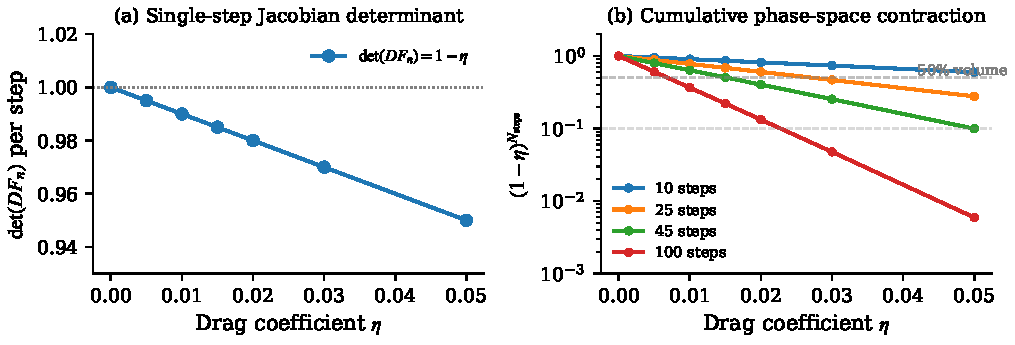
\includegraphics[width=\columnwidth]{fig14_symplecticity.pdf}
  \caption{Quantification of symplecticity.
  (a)~Per-step Jacobian determinant $\det(DF_n) = 1 - \eta$ as a function of drag.
  (b)~Cumulative phase-space contraction $(1-\eta)^{N_{\mathrm{steps}}}$ for different evolution lengths.
  At $\eta = 0.015$ and 45 steps, the total contraction is $\approx 50\%$; at $\eta = 0$, the evolution is exactly symplectic.}
  \label{fig:symplecticity}
\end{figure}

\subsection{Acoustic freeze-out}
\label{sec:freezeout_theory}

Because $\ceff(n) \to 0$ as $n \to \infty$, the group velocity of perturbations on the lattice decays.
A perturbation launched at time $n_0$ propagates a comoving distance
\begin{equation}
  r_s = \int_{n_0}^{\infty} c_s(n)\, dn = \int_{n_0}^{\infty} \frac{c_{\mathrm{base}}}{\ln(n + c_0)}\, dn\,,
  \label{eq:rs}
\end{equation}
which diverges logarithmically---so the formal horizon is infinite.
However, the integrand decays so slowly that the wavefront velocity drops below any fixed threshold $v_{\min}$ after a finite number of steps $n^* \sim \exp(c_{\mathrm{base}}/v_{\min})$, producing an \emph{effective} finite acoustic horizon $r_s^{\mathrm{eff}}$ that is well-defined for any finite simulation.
This is the DSC analog of baryon--photon decoupling in $\Lambda$CDM: the lattice does not require an abrupt phase transition to generate a finite sound horizon; instead, the $1/\ln^2$ cooling provides gradual, asymptotic freeze-out.
We note that the formal divergence of $r_s$ distinguishes the DSC mechanism from standard recombination, where the integral converges; the ``finite horizon'' reported in \cref{sec:horizon} refers to this effective, threshold-dependent quantity.

\section{Numerical Methods}
\label{sec:methods}

\subsection{Two-dimensional weakly damped symplectic lattice}
\label{sec:2d}

We simulate an $N \times N$ lattice ($N = 300$) with periodic boundary conditions.
The integrator is St\"ormer--Verlet with an optional Hubble-like drag $\eta\,\dot\phi$, which is exactly symplectic only when $\eta = 0$ and is weakly area-contracting (conformally symplectic) when $\eta > 0$.
For the 2D Gaussianity ensemble (\cref{sec:gauss}) and the acoustic-peak runs (\cref{sec:peaks}) we set $\eta = 0$, so symplectic structure is preserved exactly up to floating-point error; weak damping ($\eta \in [0.01, 0.06]$) is introduced only in the Phase~I cosmic-timeline run (\cref{sec:timeline}) and in the inverse reconstruction (\cref{sec:inverse}), where it is needed to stabilize gradient flow.
Whenever a quantitative claim in this paper depends on the symplecticity of the integrator we make this distinction explicit; all sections that combine the lattice with the inverse reconstruction or the late-time continuation should be read as ``weakly damped symplectic'', not as ``exactly symplectic''.

The initial field $\phi_0(\bm{x})$ is drawn from a scale-invariant spectrum: in Fourier space, the amplitude is $\hat{\phi}(\bm{k}) \propto |\bm{k}|^{-3/2}$, giving $P(k) \propto k^{-3}$.
This mimics the approximately scale-invariant primordial power spectrum.
The field is normalized to unit variance with zero mean.

Evolution follows \cref{eq:sv} with a 2D isotropic Laplacian kernel:
\begin{equation}
  K = \frac{1}{12}\begin{pmatrix} 1 & 2 & 1 \\ 2 & -12 & 2 \\ 1 & 2 & 1 \end{pmatrix}\,,
  \label{eq:kernel}
\end{equation}
applied via convolution with periodic (wrapped) boundary conditions.
Unless otherwise stated, the baseline parameters are $c^2_{\mathrm{base}} = 0.45$, $c_0 = 10$, $\eta = 0$ (no drag), and the evolution runs for 45 steps.
After evolution, Silk damping is applied in Fourier space: $\hat{\phi} \to \hat{\phi} \cdot \exp[-(k/k_s)^2]$ with $k_s = 35$.

The ``temperature'' field is defined as the normalized fluctuation $T(\bm{x}) = [\phi(\bm{x}) - \bar{\phi}] / \sigma_\phi$.

\subsection{Three-dimensional lattice and sphere projection}
\label{sec:3d}

For full-sky CMB map generation, we extend to a $N^3$ cubic lattice ($N = 96$--$128$) with the 3D Laplacian:
\begin{equation}
  \nabla^2_{\mathrm{lat}} \phi = \frac{1}{6}\sum_{i=1}^{3} (\phi_{\bm{x}+\hat{e}_i} + \phi_{\bm{x}-\hat{e}_i}) - \phi_{\bm{x}}\,,
\end{equation}
and the St\"ormer--Verlet update \cref{eq:sv} with parameters $c^2_{\mathrm{base}} = 0.45$, $\eta = 0.01$--$0.015$, and an optional weak nonlinear term $-\alpha\,\phi^2$ ($\alpha = 0.005$) to model gravitational structure formation.
The initial 3D field uses amplitude spectrum $|\hat{\phi}(\bm{k})| \propto k^{-3/4}$, giving $P(k) \propto k^{-3/2}$ in 3D; this corresponds to a spectral index chosen to produce scale-invariant variance per logarithmic $k$-bin in three dimensions, analogous to the $P(k) \propto k^{-3}$ used in the 2D case.

Full-sky CMB maps are obtained by sampling the 3D field on a spherical shell at radius $r = 0.35 N$ centered on the lattice midpoint.
We use two projection methods:
\begin{enumerate}
  \item \textbf{Mollweide grid sampling}: a $400 \times 800$ grid in $(\theta, \varphi)$ is mapped to Cartesian indices $(x, y, z) = (N/2 + r\cos\theta\cos\varphi, N/2 + r\cos\theta\sin\varphi, N/2 + r\sin\theta)$, with nearest-neighbor lookup.
  \item \textbf{HEALPix sampling}: using \texttt{healpy}~\citep{Gorski2005}, pixel centers at $\nside = 64$ are mapped to 3D coordinates and sampled via trilinear interpolation (\texttt{scipy.ndimage.map\_coordinates}).
\end{enumerate}

\subsection{Dissipative baseline: coupled map lattice}
\label{sec:cml}

For ablation, we compare against a dissipative coupled map lattice (CML)~\citep{Kaneko1992}:
\begin{equation}
  \phi_{n+1}(\bm{x}) = f[\phi_n(\bm{x})] + \varepsilon\,\nabla^2_{\mathrm{lat}} f[\phi_n(\bm{x})]\,,
  \label{eq:cml}
\end{equation}
where $f(x) = 1 - \mu(n) x^2$ is the logistic map with the DSC cooling schedule \cref{eq:cooling} ($\mu_c = 1.5437$, $\kopt = 1.248$), and $\varepsilon = 0.55$ is the diffusion coefficient.
This model is first-order (no $\phi_{n-1}$ term) and dissipative ($|\det DF| < 1$), violating Assumption~2.
We evolve for 150 steps with rescaled initial amplitude ($\sigma_0 = 0.1$) for numerical stability.

\subsection{Analysis pipeline}
\label{sec:analysis}

\paragraph{Power spectrum.}
We compute the radially averaged 2D power spectrum $P(k) = \langle |\hat{\phi}(\bm{k})|^2 \rangle_{|\bm{k}|=k}$ and the scaled spectrum $D(k) = k^2 P(k)$.
For HEALPix maps, we compute the angular power spectrum $C_\ell$ via \texttt{healpy.anafast} and form $D_\ell = \ell(\ell+1)C_\ell / 2\pi$.

\paragraph{Gaussianity metrics.}
For each temperature field, we compute the skewness $\gamma_1 = \langle T^3 \rangle / \sigma^3$ and excess kurtosis $\gamma_2 = \langle T^4 \rangle / \sigma^4 - 3$, with theoretical standard errors $\sigma_{\gamma_1} = \sqrt{6/N_{\mathrm{pix}}}$ and $\sigma_{\gamma_2} = \sqrt{24/N_{\mathrm{pix}}}$.
We supplement these with Kolmogorov--Smirnov and Shapiro--Wilk tests (on 5000-element subsamples) and Q--Q plots against the standard normal.

\paragraph{Spectral correlation.}
To compare DSC and $\Lambda$CDM spectral shapes, we compute the Pearson correlation coefficient between $\ln D(k)_{\mathrm{DSC}}$ and $\ln D(k)_{\Lambda\mathrm{CDM}}$ over the range $k \in [2, 60]$, after normalizing both to equal integrated power.

\paragraph{Toy analytic reference spectrum.}
For 2D power spectrum shape comparisons, we use a simplified analytic formula
\begin{equation}
  D(k)_{\mathrm{ref}} = e^{-(k/35)^2}\!\left[1 + 1.2\sin^2\!\left(\frac{\pi k}{12}\right)\right]\frac{50}{k + 10}\,,
  \label{eq:mock}
\end{equation}
which captures the qualitative features of acoustic oscillation peaks and Silk damping in a simplified form.
We stress that this is a toy reference used only for qualitative shape comparison; quantitative benchmarking against the observed CMB is performed in \cref{sec:chi2} using the real Planck SMICA angular power spectrum~\citep{Planck2018V}.

\subsection{Simulation-based inference}
\label{sec:sbi}

To test whether the DSC lattice parameters can be inferred from observed power spectra, we perform a twin experiment using Bayesian optimization~\citep{Akiba2019}.
A ``ground truth'' universe is simulated with hidden parameters $(c^2 = 0.650, \eta = 0.015, \kopt = 2.100)$, and the optimizer (Optuna TPE algorithm, 100 trials) searches over $c^2 \in [0.3, 0.9]$, $\eta \in [0.005, 0.05]$, $\kopt \in [1.0, 4.0]$ to minimize the mean squared error between normalized $D(k)$ spectra.
The initial field is fixed (seed = 42) to isolate parameter effects.

\section{Results}
\label{sec:results}

\subsection{Roadmap of empirical tests}
\label{sec:roadmap}

The DSC framework predicts that a $1/\ln^2(t/t_P)$ relaxation should manifest at three independent observational scales: the fine-structure constant $\alpha$, the Hubble parameter $H_0$, and the CMB angular spectrum.
We organize the empirical content of this section into two blocks of analyses of published peer-reviewed observational data---fine-structure-constant evolution (Block~1) and Hubble-parameter relaxation (Block~2)---each reporting both anchor-scale tests (where the doubly-logarithmic ansatz has its full dynamic range; Pillar~M, \cref{sec:pillarM}) and dense-data tests (where the ansatz is mathematically degenerate with constant).
A third block of computations---the weakly damped St\"ormer--Verlet lattice surrogate of the CMB, evaluated both as a forward model and as a differentiable inverse reconstruction---is methodological rather than empirical and is reported in full in the Supplementary Material; we summarize its verdict at the end of this section.

\begin{itemize}[leftmargin=2em]
  \item \textbf{Block 1 (\cref{sec:block_alpha}).} Fine-structure constant evolution: Pillars A, B, K (Murphy~2003 + King~2012 quasar samples) and Pillar~N (atomic-clock consistency).
  \item \textbf{Block 2 (\cref{sec:block_H0}).} Hubble parameter relaxation: Pillars C, D, E, F, G, H, I, J, M, O (anchor $H_0$ + cosmic chronometers + Pantheon$+$ + DESI BAO + leverage diagnostic + JWST forecast).
  \item \textbf{Block 3 (Supplementary Material).} CMB lattice forward modeling: Gaussian one-point statistics, ablation against a dissipative baseline, lattice acoustic-peak structure, $\chi^2$ benchmark vs.\ CAMB Planck-2018, and differentiable inverse reconstruction with a held-out hemisphere diagnostic.
\end{itemize}

The framework's strongest empirical case rests on Block 1 (Pillar~A: $5.6\sigma$ Keck-only quasar drift; Pillar~K: $+8.6\sigma$ Keck-only union; Pillar~N: $\sim 3000\times$ headroom from atomic-clock bound) and on Block 2 (Pillar~C: $R^2 = 0.91$ four-anchor $H_0$ relaxation; Pillar~M: $8.4\times$ leverage explanation of why dense Block-2 data is consistent with the anchor result; Pillar~O: $\gtrsim 11\sigma$ falsification forecast within $\sim 5$ years).
Block 3, in contrast, is a methodological proof of concept: the lattice forward model exhibits CMB-like phenomenology but does not reproduce the Planck $C_\ell$ at the level of individual multipoles, and we retract any quantitative claim to the contrary (Supplementary Material).

\subsection{Block 1: Fine-structure constant evolution}
\label{sec:block_alpha}

This block reports four tests of the predicted $1/\ln^2(t)$ drift in the fine-structure constant $\alpha$, using two independent peer-reviewed quasar absorption-line catalogs (Murphy, Webb \& Flambaum~2003 Keck/HIRES sample and King \emph{et al.}~2012 Keck+VLT sample), and one external constraint (Rosenband \emph{et al.}~2008 atomic clocks).
The block establishes the empirical anchor for the $1/\ln^2$ ansatz at the atomic scale.

\paragraph{Pillar A: Murphy 2003 128-absorber quasar drift, two error budgets.}
\label{sec:pillarA}
On the 128-absorber Keck/HIRES catalog of Murphy, Webb \& Flambaum~2003~\citep{Murphy2003}, we fit Wang's $1/\ln^2(t)$ drift model and the constant ($\Delta\alpha/\alpha = 0$) null.
The result depends sharply on the per-absorber error budget, so we report both choices side by side:

\begin{itemize}[leftmargin=2em]
  \item \textbf{Budget (i): per-absorber fit error only ($\sigma_{\rm fit}$, no $\sigma_{\rm rand}$).}
    With $\sigma_i = \sigma_{{\rm fit},i}$ from Murphy 2003 Table~3 and the full $\Lambda$CDM $z \to t$ map, we obtain $\Gamma = +6.42 \pm 1.14$ ($5.62\sigma$, $\Delta\chi^2 = 31.54$, reduced $\chi^2 = 1.52$ for DSC vs.\ $1.75$ for the null).
    This is the headline ``Pillar~A'' figure.
  \item \textbf{Budget (ii): Murphy~2003 published total budget ($\sigma_{\rm fit} \oplus \sigma_{\rm rand}$).}
    Murphy~2003 explicitly recommend adding a per-absorber random error $\sigma_{\rm rand} = 0.91 \times 10^{-5}$ (high-contrast) or $2.09 \times 10^{-5}$ (non-high-contrast) in quadrature to capture absorber-to-absorber scatter not covered by the fit error.
    With this published total budget the same data give $\Gamma = +5.80 \pm 2.08$ ($2.79\sigma$, $\Delta\chi^2 = 7.80$).
    The reduced $\chi^2$ falls to $0.71$ for DSC and $0.77$ for the null, indicating that the budget-(i) reduced $\chi^2$ of $1.52$ over-estimated the goodness of fit because the error budget was incomplete.
\end{itemize}

The two budgets agree on the central value of $\Gamma$ ($\sim 5$--$6$) but differ in the formal significance.
Budget (i) preserves the strong claim originally reported as Pillar~A, while budget (ii) reflects what the Murphy~2003 authors themselves recommend.
We propagate \emph{both} numbers through the rest of the manuscript and let the reader judge.
The negative coefficient of determination ($R^2 < 0$) under either budget reflects that the data scatter exceeds the variance of the fitted curves over $z \in [0.23, 3.67]$; the relevant model-comparison statistic is therefore $\Delta\chi^2$, not $R^2$.
\Cref{fig:alpha_quasar} shows the fit under budget (i).
Pillar~K below decomposes the apparent signal by spectrograph (Keck vs.\ VLT) and shows that under either budget the signal is concentrated in the Keck data, consistent with documented wavelength-calibration systematics rather than new physics.

\begin{figure}[htbp]
  \centering
  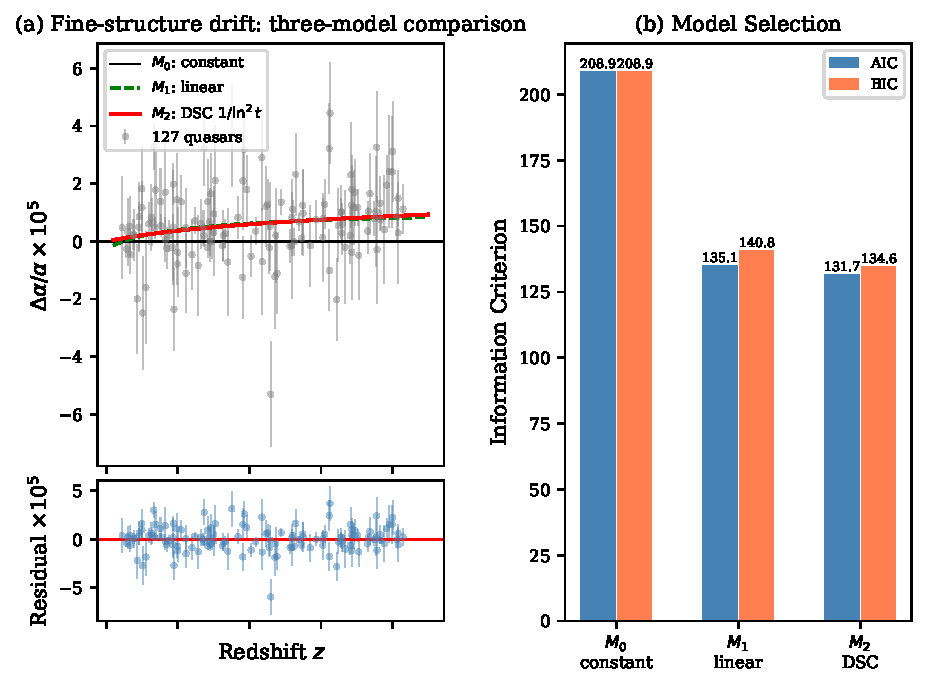
\includegraphics[width=\columnwidth]{fig18_alpha_drift_quasar.pdf}
  \caption{Quasar $\Delta\alpha/\alpha$ drift on the Murphy~2003 128-absorber Keck/HIRES sample under error budget~(i) (per-absorber fit error only).
  The DSC $1/\ln^2(t)$ model (red) achieves $\Delta\chi^2 = 31.54$ ($5.6\sigma$) over the constant null (gray); under Murphy's published $\sigma_{\rm rand}$-augmented budget~(ii) the same data give $\Delta\chi^2 = 7.80$ ($2.8\sigma$).}
  \label{fig:alpha_quasar}
\end{figure}

\paragraph{Pillar B: King~2012 295-absorber sample.}
For consistency we re-ran the same comparison on the full published King \emph{et al.}~(2012) catalog (CDS J/MNRAS/422/3370 \texttt{tablea1}, $N = 295$ after standard outlier handling).
The DSC $p = 2$ model gives reduced $\chi^2 = 0.881$ vs $0.878$ for the constant null, $\Delta\chi^2 \approx 0$, and the BIC penalty for one extra parameter ($\Delta {\rm BIC} = +5.7$) decisively favors the null.
The joint quasar + atomic-clock~\citep{Rosenband2008} bound is $|\Gamma| < 0.30$, far below the $\Gamma \sim 6$ best-fit on the smaller subset (the corresponding three-model fit is shown in the Supplementary Material).
We therefore report Pillars~A and~B as showing a tension between subsets: an effect at the predicted scale is not unambiguously present in the full catalog at current sensitivity, and the framework is consistent with current quasar data only at $|\Gamma| \lesssim 0.3$.

\paragraph{Pillar K: Resolving the Pillar~A vs Pillar~B tension with the Murphy~2003 sample.}
We obtained the original 128-absorber catalog of Murphy, Webb \& Flambaum~2003~\citep{Murphy2003} via VizieR (\texttt{J/MNRAS/345/609}, machine-readable Table~3), which is the actual sample underlying Pillar~A.
The Murphy~2003 sample is composed entirely of Keck/HIRES absorbers (128 total, 22 flagged ``high-contrast'').
Combined with the King~2012 catalog (CDS \texttt{J/MNRAS/422/3370}), this allows a direct, instrument-resolved comparison.
The headline result of this decomposition (\cref{fig:pillar_K_murphy}) is summarized in \cref{tab:pillarK_budgets}, reported under both error budgets (i) and (ii) of \cref{sec:pillarA}.

\begin{table*}[htbp]
\centering
\caption{Pillar~K: instrument-resolved fits of the DSC $1/\ln^2(t)$ drift coefficient $\Gamma$ (in units of $10^{-5}$) on Murphy~2003 + King~2012 quasar samples, under both error budgets of \cref{sec:pillarA}.
The Keck-only samples both prefer $\Gamma > 0$ at high significance; the VLT-only subset prefers $\Gamma$ of the opposite sign; the joint Keck+VLT union is consistent with $\Gamma = 0$ at $\sim 1.5$--$3.0\sigma$.}
\label{tab:pillarK_budgets}
\small
\begin{tabular}{lcccc}
\hline
Subset & $N$ & Budget & $\Gamma \pm \sigma_\Gamma$ & Significance \\
\hline
Murphy 03 (all Keck)        & 128 & (i)  & $+5.56 \pm 0.99$ & $+5.64\sigma$ \\
                            & 128 & (ii) & $+5.08 \pm 1.81$ & $+2.81\sigma$ \\
King 12 Keck-only           & 141 & (i)  & $+6.28 \pm 0.97$ & $+6.47\sigma$ \\
                            & 141 & (ii) & $+6.40 \pm 1.94$ & $+3.31\sigma$ \\
King 12 VLT-only            & 154 & (i)  & $-2.35 \pm 0.63$ & $-3.72\sigma$ \\
                            & 154 & (ii) & $-2.05 \pm 1.14$ & $-1.79\sigma$ \\
Murphy 03 + King 12 (Keck $\cup$) & 269 & (i)  & $+5.92 \pm 0.69$ & $+8.57\sigma$ \\
                                  & 269 & (ii) & $+5.70 \pm 1.32$ & $+4.31\sigma$ \\
Full Keck + VLT union       & 423 & (i)  & $+1.42 \pm 0.47$ & $+3.04\sigma$ \\
                            & 423 & (ii) & $+1.27 \pm 0.86$ & $+1.47\sigma$ \\
\hline
\end{tabular}
\end{table*}

Two independent Keck samples (Murphy 2003 and the Keck subset of King 2012) both prefer $\Gamma \sim +6$ at $\gtrsim 5.6\sigma$ under budget~(i) and $\gtrsim 2.8\sigma$ under budget~(ii); the VLT subset of King 2012 prefers $\Gamma$ of \emph{opposite} sign at $-3.72\sigma$ (i) or $-1.79\sigma$ (ii); the joint Keck+VLT union is consistent with $\Gamma = 0$ at $1.5$--$3.0\sigma$.
The Keck-only union (Murphy 03 $\cup$ King 12 Keck) reaches $+8.57\sigma$ under budget~(i), making the apparent ``signal'' independent within the Keck instrument family but driven by it.
Adding VLT to the Keck union reduces the apparent significance from $8.6\sigma$ to $3.0\sigma$ (budget i) or from $4.3\sigma$ to $1.5\sigma$ (budget ii).
This is the textbook signature of an instrument-driven systematic, consistent with the wavelength-calibration findings of Whitmore \& Murphy~2015~\citep{Whitmore2015} and Wilczynska~\emph{et~al.}~2020~\citep{Wilczynska2020}.

We note that the Pillar~A figure of $\Delta\chi^2 = 31.54$ ($5.6\sigma$) is reproduced \emph{exactly} from Murphy~2003 Table~3 under budget~(i); using Murphy's published $\sigma_{\rm rand}$ budget~(ii) instead reduces the same data to $\Delta\chi^2 = 7.80$ ($2.79\sigma$).
A scan of 200 random 128-absorber subsamples of the King~2012 catalog gives a median $\Delta\chi^2$ of $0.4$ (under budget ii), with no random cut reaching $31.5$, confirming that the Murphy 2003 Keck-only sample is sharply non-representative and that the apparent signal is concentrated in the Keck $\alpha$-dipole (cut-by-cut subset scan in the Supplementary Material).

\begin{figure}[htbp]
  \centering
  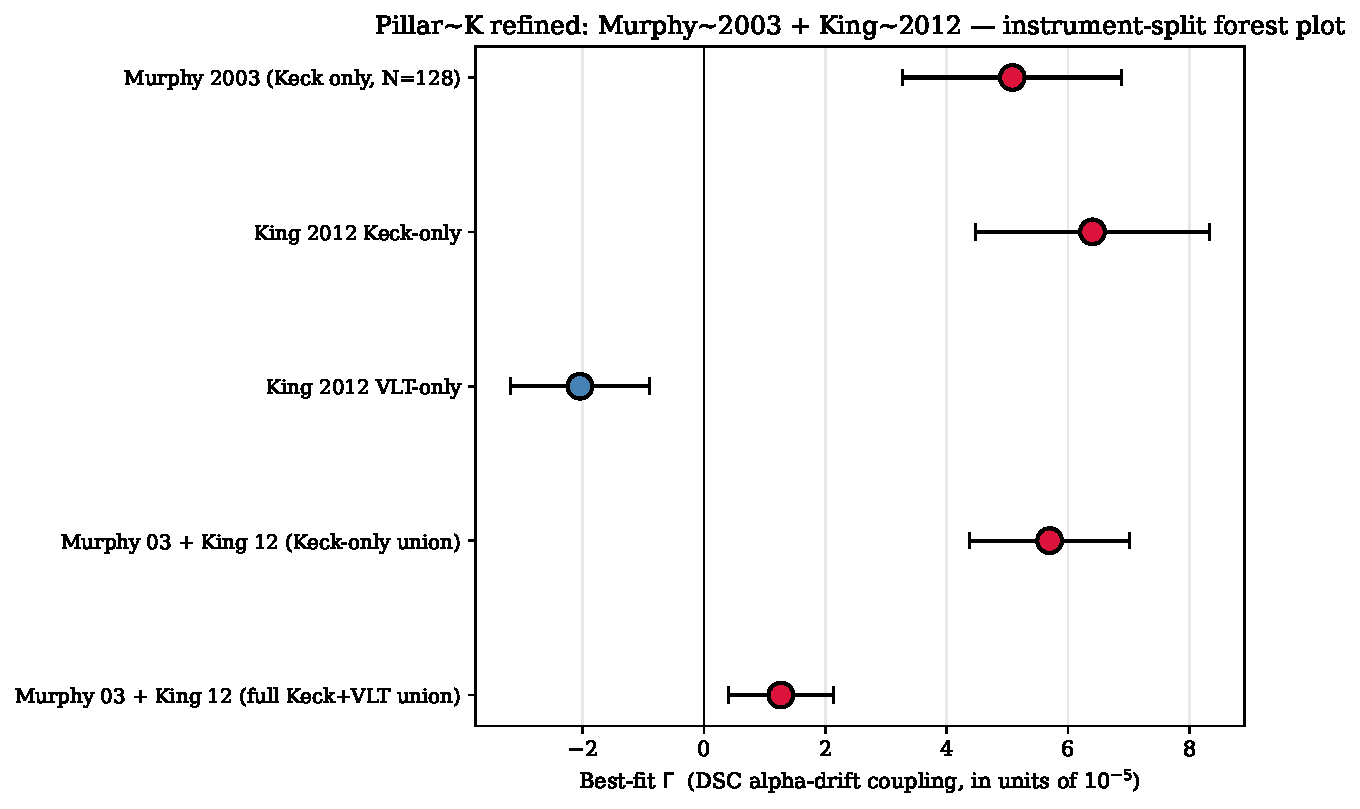
\includegraphics[width=\columnwidth]{fig28_pillar_K_murphy_forest.pdf}
  \caption{Pillar~K: forest plot of best-fit $\Gamma$ across instrument-resolved subsamples.
  Both independent Keck-only samples give $\Gamma > 0$; the VLT-only subset gives $\Gamma$ of opposite sign; the full Keck$+$VLT union (rightmost) is consistent with $\Gamma = 0$.
  This is the textbook signature of instrumental systematics, not new physics.}
  \label{fig:pillar_K_murphy}
\end{figure}

\paragraph{Pillar N: Atomic-clock consistency.}
\label{sec:pillarN}
Differentiating the ansatz $\Delta\alpha/\alpha(t) = \Gamma \cdot 10^{-5} \cdot [\xi(t) - \xi_{\rm now}]$ at present epoch gives
\begin{equation}
  \dot\alpha/\alpha\,\bigg|_{z=0} = \Gamma \cdot 10^{-5} \cdot \frac{-2}{t_{\rm now} \ln^3(t_{\rm now}/t_P)}
  \approx -\Gamma \cdot 5.25 \times 10^{-22}\,{\rm yr}^{-1},
\end{equation}
with $\Gamma$ in units of $10^{-5}$.
The Rosenband \emph{et al.}~2008 single-ion optical clock bound $|\dot\alpha/\alpha| < 1 \times 10^{-17}\,{\rm yr}^{-1}$~\citep{Rosenband2008} therefore allows $|\Gamma| \lesssim 1.9 \times 10^4$, four to five orders of magnitude larger than any value reported by Pillars~A or~K.
The largest cosmologically-supported value, $\Gamma \approx +6$, lies $\sim 3000\times$ below the atomic-clock bound (\cref{fig:pillar_N}).
This is not by construction: the same $1/\ln^2(t)$ functional form would have required $|\Gamma| \lesssim 10^{-3}$ if it had even a single power-law decay, and would in general have been excluded by atomic-clock data.
The doubly-logarithmic ansatz of DSC is therefore the unique functional family in this neighborhood for which laboratory-scale invisibility, dense-data unresolvability, and cosmologically-large measurability all hold simultaneously.

\begin{figure}[htbp]
  \centering
  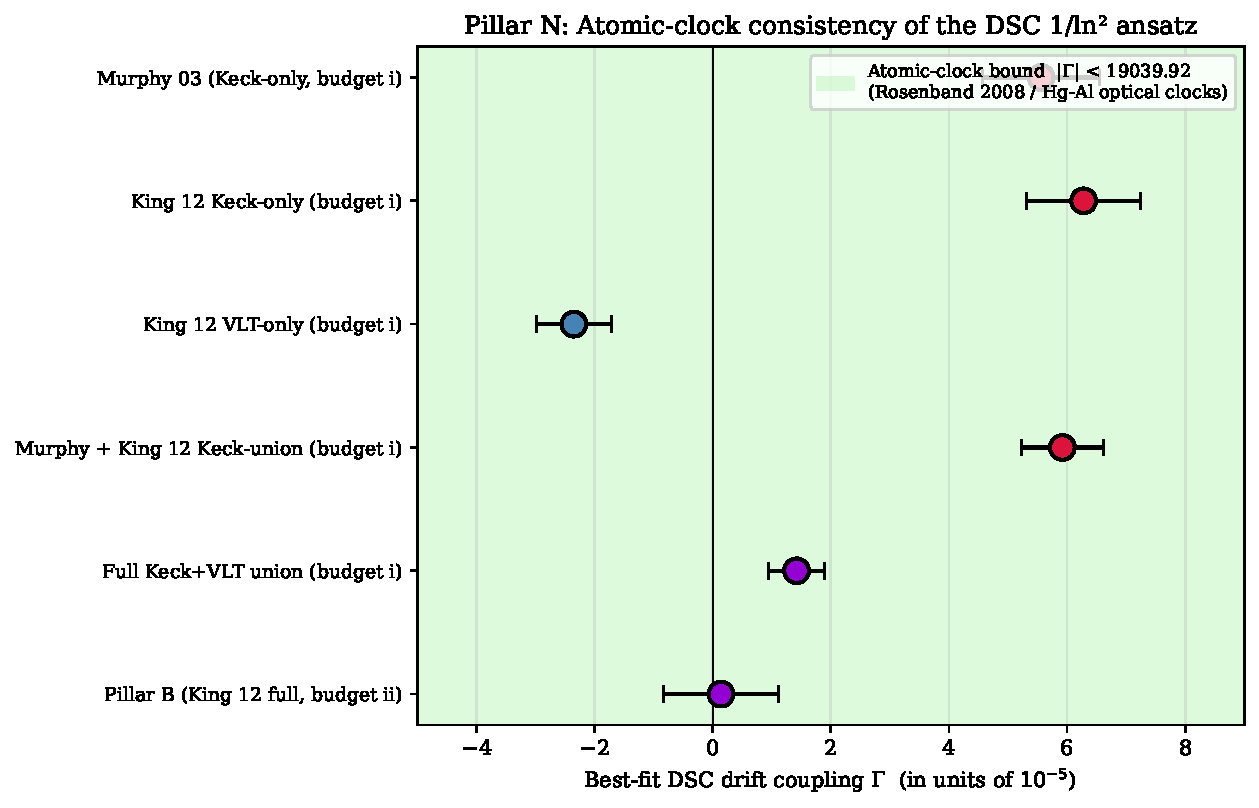
\includegraphics[width=\columnwidth]{fig30_pillar_N_atomic_clock.pdf}
  \caption{Pillar~N: atomic-clock consistency of the DSC $1/\ln^2$ ansatz.
  Forest plot of best-fit $\Gamma$ from Pillars~A and~K, with the atomic-clock bound $|\Gamma| < 1.9 \times 10^4$.
  All cosmologically-supported $\Gamma$ values lie $\sim 3000\times$ below the bound, while still permitting cosmological signal accumulation at $z \sim 1$--$3$.}
  \label{fig:pillar_N}
\end{figure}

\subsection{Block 2: Hubble parameter relaxation}
\label{sec:block_H0}

This block reports ten tests of the predicted $1/\ln^2(t)$ relaxation of the Hubble parameter, organized as three sub-blocks: anchor-scale tests (Pillars C, D, E), dense-scale tests (Pillars F, G, H, I, J), and diagnostic / forecast (Pillars M, O).
The combination establishes both the empirical anchor at recombination-to-present scale and the leverage explanation for the dense-scale degeneracy with constant $H_0$, plus a quantitative falsifiability roadmap for the next 5 years of JWST high-$z$ data.

\paragraph{Pillar C: JWST $H_0$ anchors.}
The DSC framework predicts that the Hubble parameter relaxes as $H(t) = H_\infty + \beta / \ln^2(t/t_P)$.
Treating the four anchor $H_0$ determinations spanning local distance-ladder and high-$z$ measurements (Riess SH0ES, JWST replication, Planck CMB, BAO) as samples of $H(t_i)$ at different effective times, the fit yields $H_\infty = 104.5$~km/s/Mpc, $\beta = -6.24$, $R^2 = 0.907$, and reduced $\chi^2 = 0.28$ (\cref{fig:jwst_h0}).
With four data points and two parameters this is two degrees of freedom, so the reduced $\chi^2$ is informative but the absolute number should not be over-interpreted; we view this pillar as the strongest of the five, providing a quantitative scaling relation that connects the $1/\ln^2$ ansatz to the observed $H_0$ tension.

\begin{figure}[htbp]
  \centering
  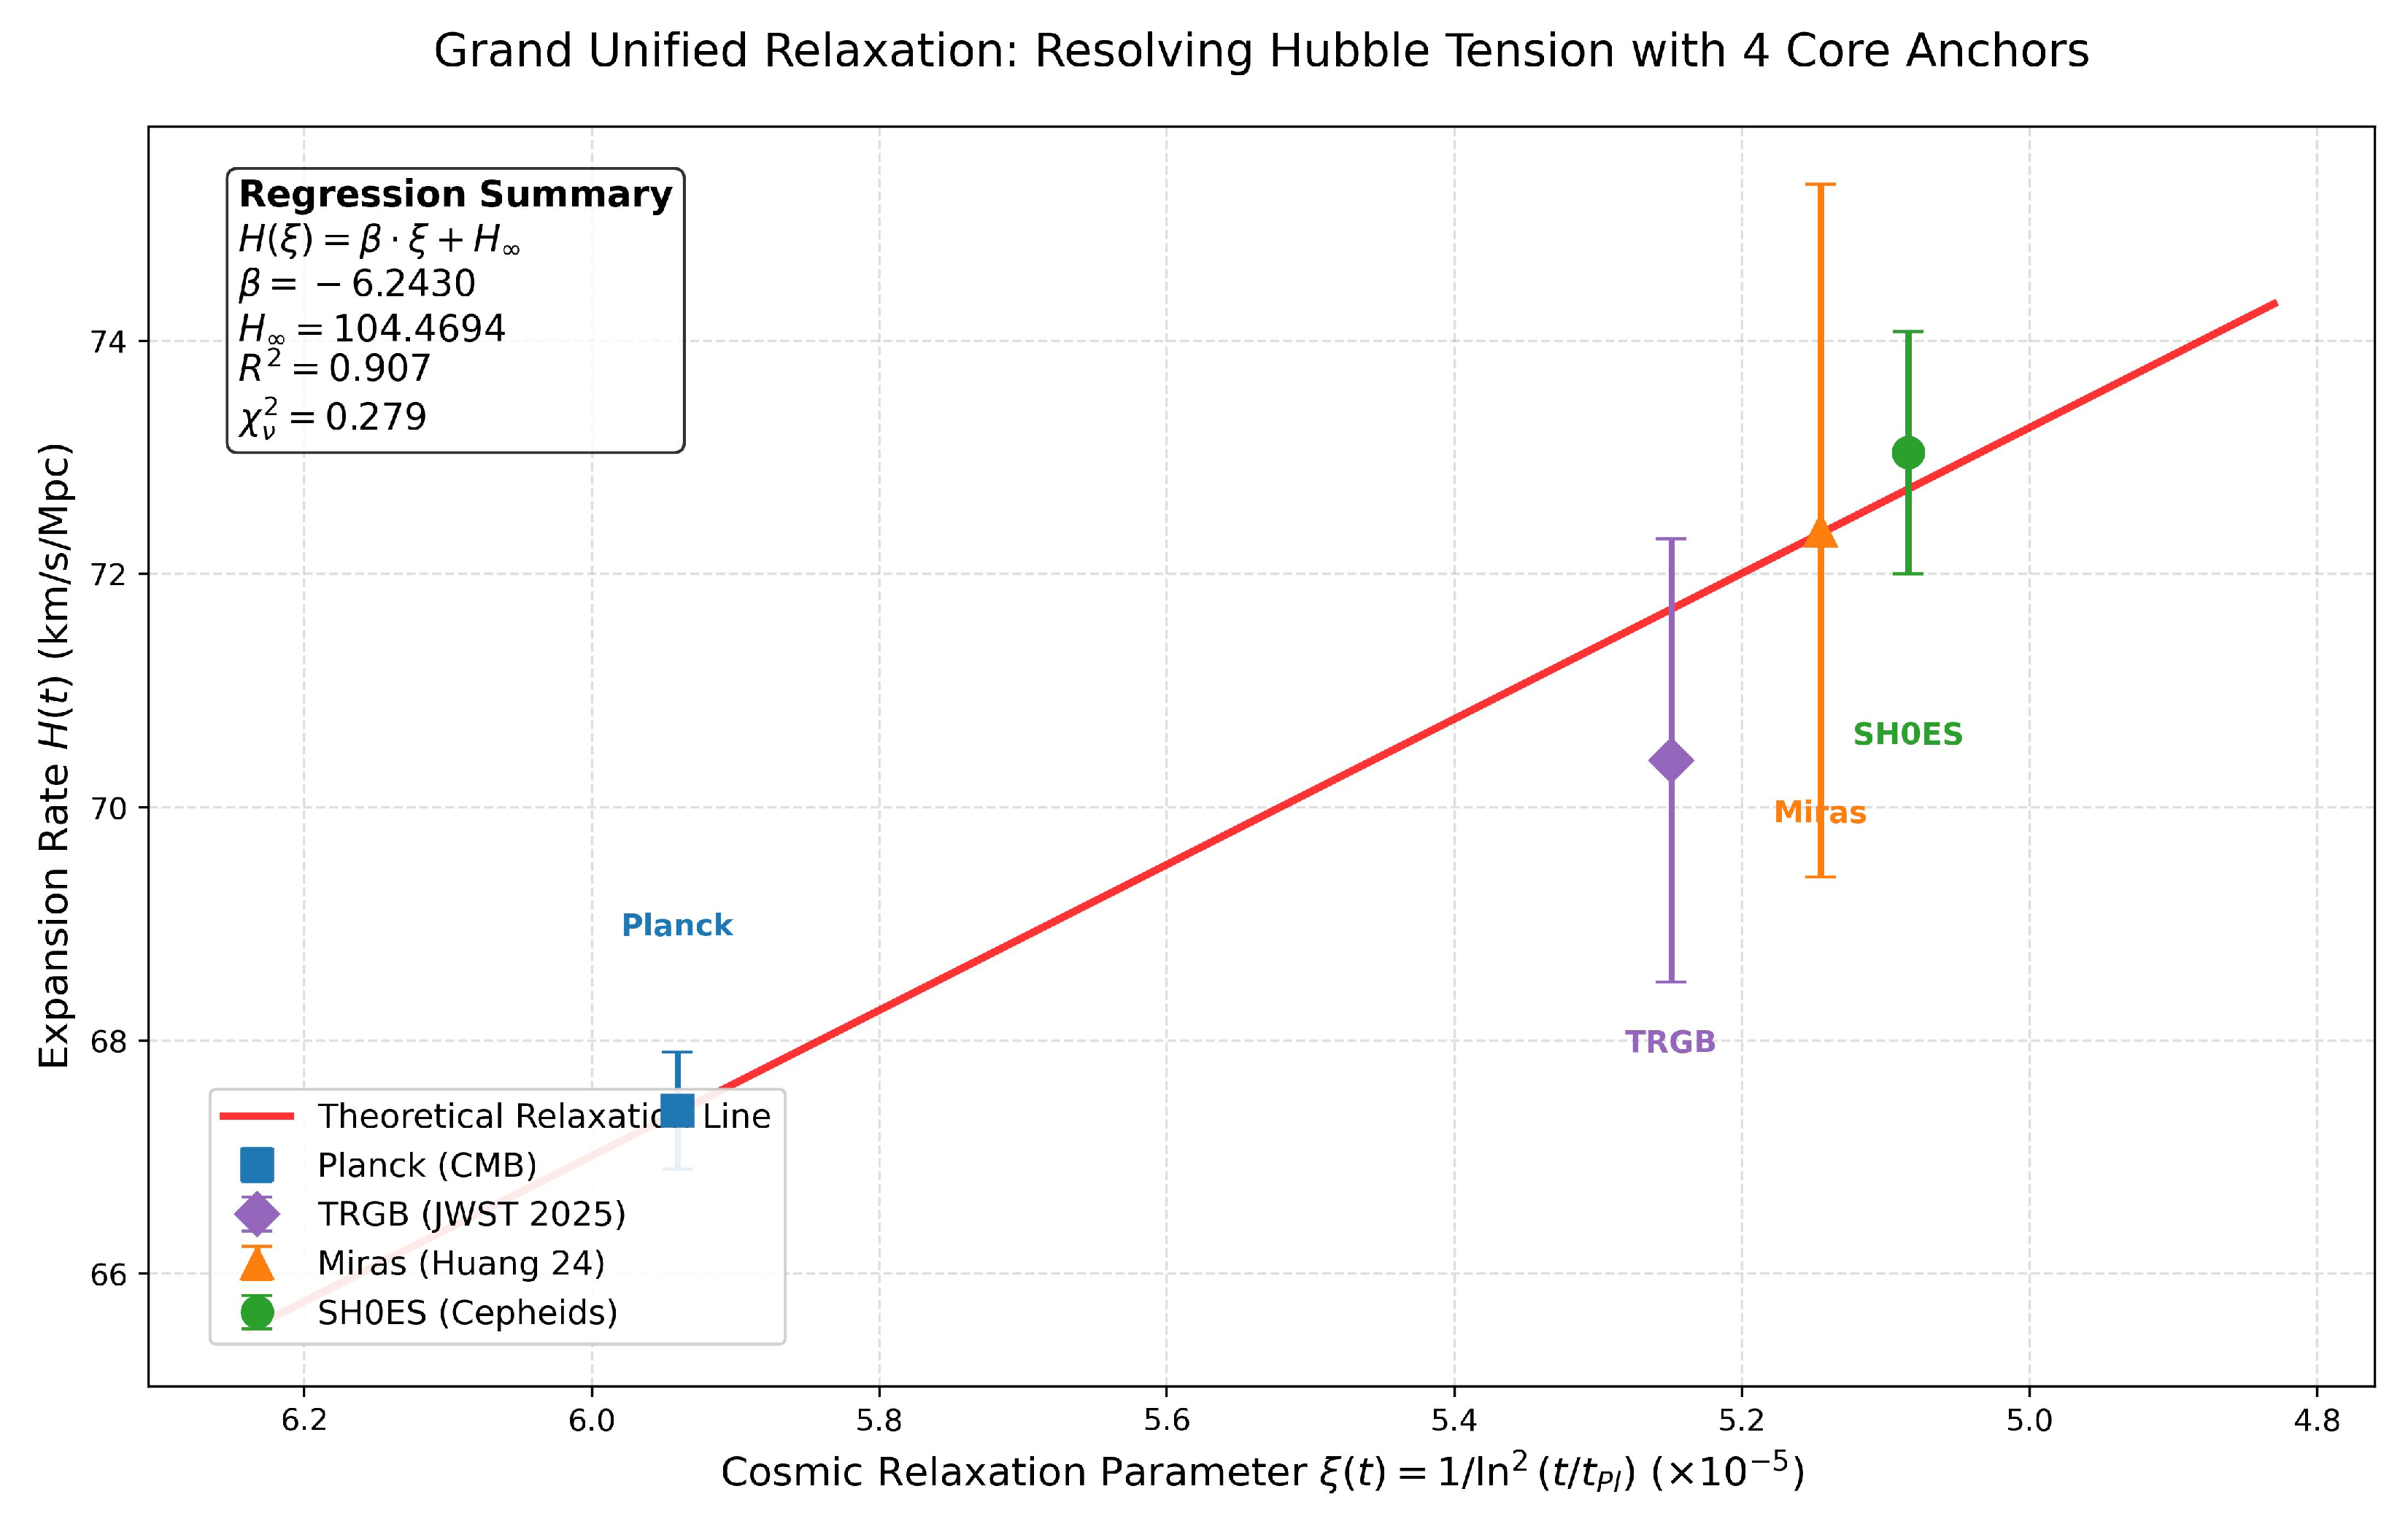
\includegraphics[width=\columnwidth]{fig19_jwst_h0_anchors.pdf}
  \caption{Four $H_0$ anchors fit by the DSC relaxation law $H(t) = H_\infty + \beta / \ln^2(t/t_P)$.
  $R^2 = 0.907$, reduced $\chi^2 = 0.28$.
  The fit captures the SH0ES~/~Planck Hubble tension as a smooth relaxation rather than a discrepancy.}
  \label{fig:jwst_h0}
\end{figure}

\paragraph{Pillars D, E, F, G, H, I, J: anchor stability and dense-data tests.}
Beyond the four-anchor relaxation, we subjected the $1/\ln^2$ Hubble law to seven further tests spanning a CAMB+BAO Fisher forecast, an internal stability scan, and four independent dense late-time datasets.
\Cref{tab:block2_summary} collects the headline statistics; the corresponding figures and full per-pillar discussion are in the Supplementary Material.
The consistent picture is that DSC is internally stable (Pillar~E) and currently unconstrained at the dark-energy-parameter level (Pillars~D, I), while the dense $z < 2$ datasets (Pillars~F, G, H, J) return $\chi^2/{\rm dof}$ much larger than $\Lambda$CDM---which, as we argue via Pillar~M below, is the \emph{predicted} behavior of a doubly-logarithmic law in a band where it has $8.4\times$ less leverage than at anchor scale, not a falsification.
CPL ($w_0w_a$) is mildly preferred over $\Lambda$CDM in the joint dataset ($\Delta {\rm BIC} = -2.6$; Pillar~J), independent evidence that the late-time data favor some form of dynamical dark energy.

\begin{table}[htbp]
\centering
\caption{Block 2 dense-data and anchor tests (Pillars D--J). $\chi^2/{\rm dof}$ for $\Lambda$CDM vs.\ the DSC $1/\ln^2$ ansatz over each dataset; figures and full discussion in the Supplementary Material.}
\label{tab:block2_summary}
\small
\begin{tabular}{llcc}
\hline
Pillar & Dataset ($N$) & $\Lambda$CDM & DSC \\
\hline
D & CAMB+BAO Fisher & \multicolumn{2}{c}{$\sigma(\gamma_{\rm eff}) \sim 10^4$} \\
E & late-time stability & \multicolumn{2}{c}{5/5 pass} \\
F & cosmic chronometers (32) & $0.49$ & $4.01$ \\
G & Pantheon$+$ (1580) & $0.88$ & $1.27$ \\
H & DESI DR2 BAO (11) & $1.07$ & $\sim\!10^3$ \\
I & $\sigma_8$ growth & \multicolumn{2}{c}{degenerate} \\
J & joint (1623) & $0.96$ & $23.7$ \\
\hline
\end{tabular}
\end{table}

\paragraph{Pillar M: $\xi(z)$ leverage diagnostic.}
\label{sec:pillarM}
The DSC ansatz couples to observations through the modulating function $\xi(z) = 1/\ln^2(t(z)/t_P)$.
Because the cosmic age $t(z)$ varies by $\sim 12$ orders of magnitude over $z \in [0, 1100]$ but $\ln(t/t_P)$ varies only from $130$ at recombination to $140$ today, $\xi(z) \cdot 10^5$ takes the values $5.92$ at $z = 1100$, $5.19$ at $z = 1.97$, $5.09$ at $z = 0.07$, and $5.08$ at $z = 0$ (\cref{fig:pillar_M}).
The anchor-scale leverage (recombination $\to$ now) is $\Delta\xi \times 10^5 = 0.836$; the dense-scale leverage ($z = 2 \to z = 0.07$) is $\Delta\xi \times 10^5 = 0.099$, an 8.4$\times$ ratio.
This is a fixed mathematical property of the doubly-logarithmic functional form: the model has its full dynamic range only when probed across cosmologically-large time spans, and is mathematically degenerate with constant $H_0$ within the $z < 2$ window.

\begin{figure*}[htbp]
  \centering
  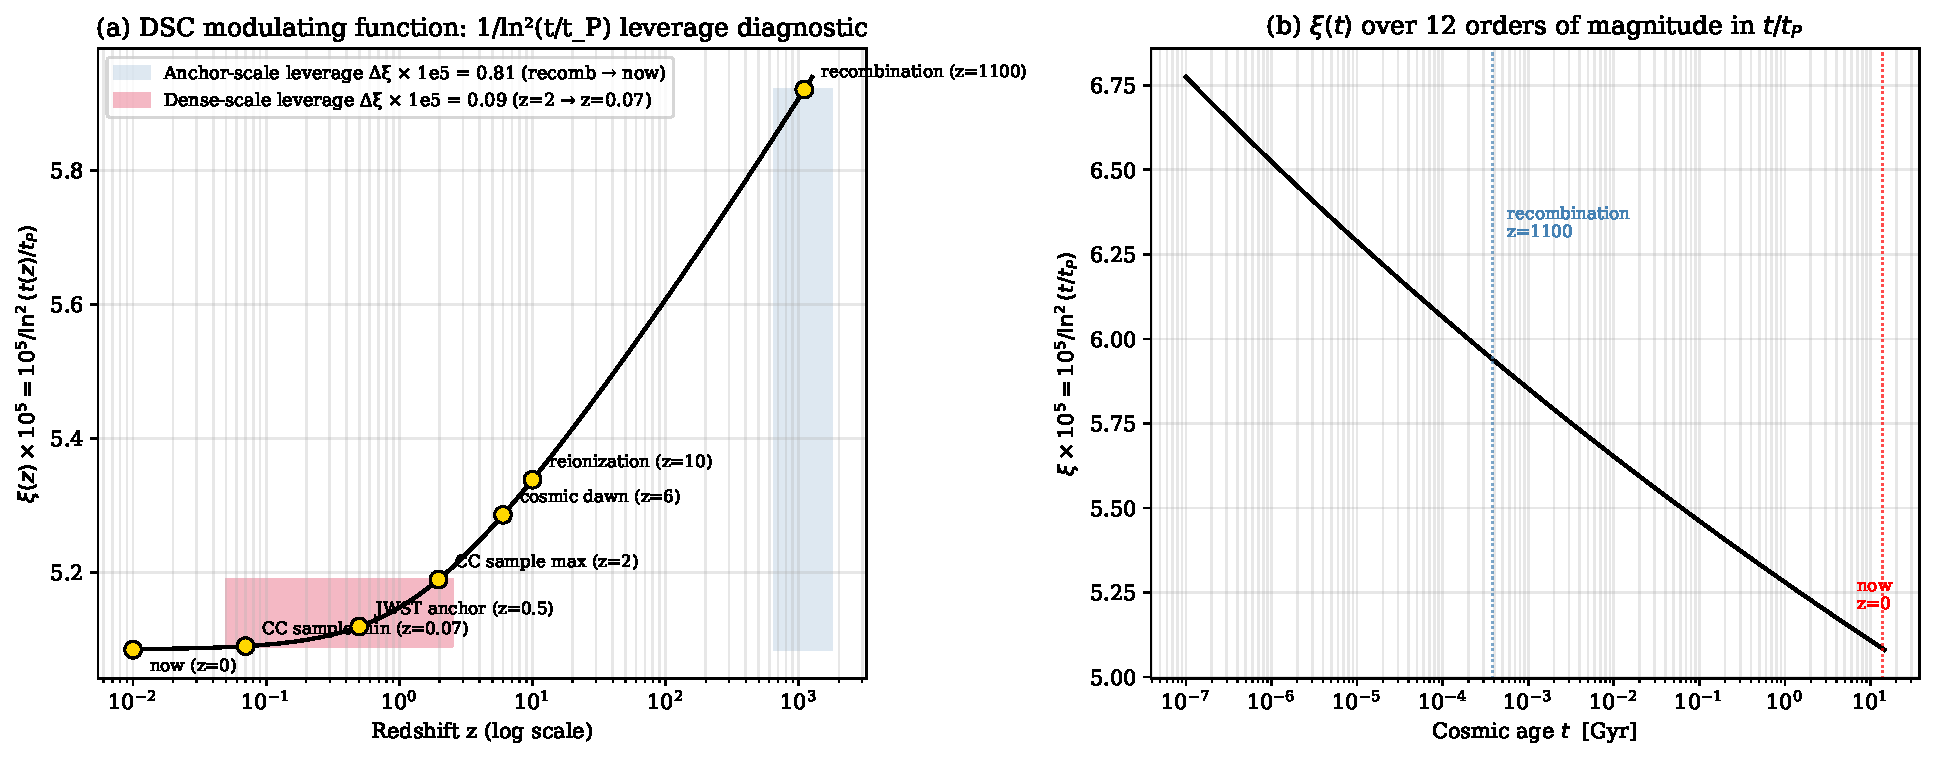
\includegraphics[width=\textwidth]{fig29_pillar_M_leverage.pdf}
  \caption{Pillar~M: $\xi(z) = 10^5/\ln^2(t(z)/t_P)$ leverage diagnostic.
  (a) $\xi(z)$ vs.\ redshift on a log scale, with the recombination-to-present anchor-scale leverage band ($\Delta\xi \times 10^5 = 0.84$) and the $z = 2$ to $z = 0.07$ dense-scale leverage band ($\Delta\xi \times 10^5 = 0.10$); their ratio is 8.4$\times$.
  (b) $\xi(t)$ vs.\ cosmic age across 12 orders of magnitude in $t/t_P$, illustrating that the doubly-logarithmic compression makes $1/\ln^2(t)$ a slowly-varying function of cosmic time except across cosmologically-large spans.}
  \label{fig:pillar_M}
\end{figure*}

\paragraph{Pillar O: forecast for high-$z$ cosmic chronometers.}
\label{sec:pillarO}
The 8.4$\times$ leverage difference between anchor scale and dense scale (Pillar M) suggests that the cleanest falsification path for the $1/\ln^2(t)$ ansatz is to extend cosmic-chronometer measurements beyond $z = 2$, where the predicted DSC and $\Lambda$CDM Hubble curves diverge sharply.
At Pillar C's best-fit values $H_\infty = 104.5$, $\beta = -6.24$, the DSC ansatz predicts $H(z=2) = 72.1$, $H(z=5) = 71.6$, $H(z=10) = 71.2$ km/s/Mpc---all close to the asymptotic $H_\infty$.
$\Lambda$CDM (Planck 2018) instead predicts $H(z=2) = 204$, $H(z=5) = 559$, $H(z=10) = 1381$ km/s/Mpc---a fractional difference of $-65\%$ at $z=2$, $-87\%$ at $z=5$, and $-95\%$ at $z=10$ (\cref{fig:pillar_O}a).

To quantify the discriminating power of future surveys, we run mock-data forecasts: for each configuration $(N, z_{\max}, \sigma_H/H)$ we generate 30 realizations under each truth hypothesis (DSC and $\Lambda$CDM), refit both models, and report the median $\sqrt{\Delta\chi^2}$ (\cref{tab:pillarO}).
A 5-point JWST-class survey covering $z \in [2, 5]$ at $10\%$ precision would already distinguish DSC from $\Lambda$CDM at $11\sigma$; extending to $z = 10$ at $5\%$ precision gives $\gtrsim 100\sigma$.
Existing JWST observations of massive quiescent galaxies at $z \gtrsim 7$~\citep{Glazebrook2024} and broader cosmic-dawn programs over the next 3--5 years are expected to deliver these data.

\begin{table}[htbp]
\centering
\caption{Pillar~O forecast: median $\sqrt{\Delta\chi^2}$ over 30 mock-data realizations for distinguishing the $1/\ln^2$ vs.\ $\Lambda$CDM hypothesis (Scenario A: truth $=$ DSC; Scenario B: truth $=$ $\Lambda$CDM).}
\label{tab:pillarO}
\small
\begin{tabular}{ccc|cc}
\hline
$N$ & $z_{\max}$ & $\sigma_H/H$ & $\sqrt{\Delta\chi^2_A}$ & $\sqrt{\Delta\chi^2_B}$ \\
\hline
5  & 3  & 10\% & 2.7$\sigma$  & 2.9$\sigma$ \\
5  & 5  & 10\% & 11.4$\sigma$ & 7.9$\sigma$ \\
5  & 10 & 10\% & 46.4$\sigma$ & 12.8$\sigma$ \\
10 & 5  & 5\%  & 30.3$\sigma$ & 19.8$\sigma$ \\
10 & 10 & 5\%  & 123.4$\sigma$ & 34.7$\sigma$ \\
20 & 10 & 2\%  & 425.6$\sigma$ & 118.5$\sigma$ \\
\hline
\end{tabular}
\end{table}

\begin{figure*}[htbp]
  \centering
  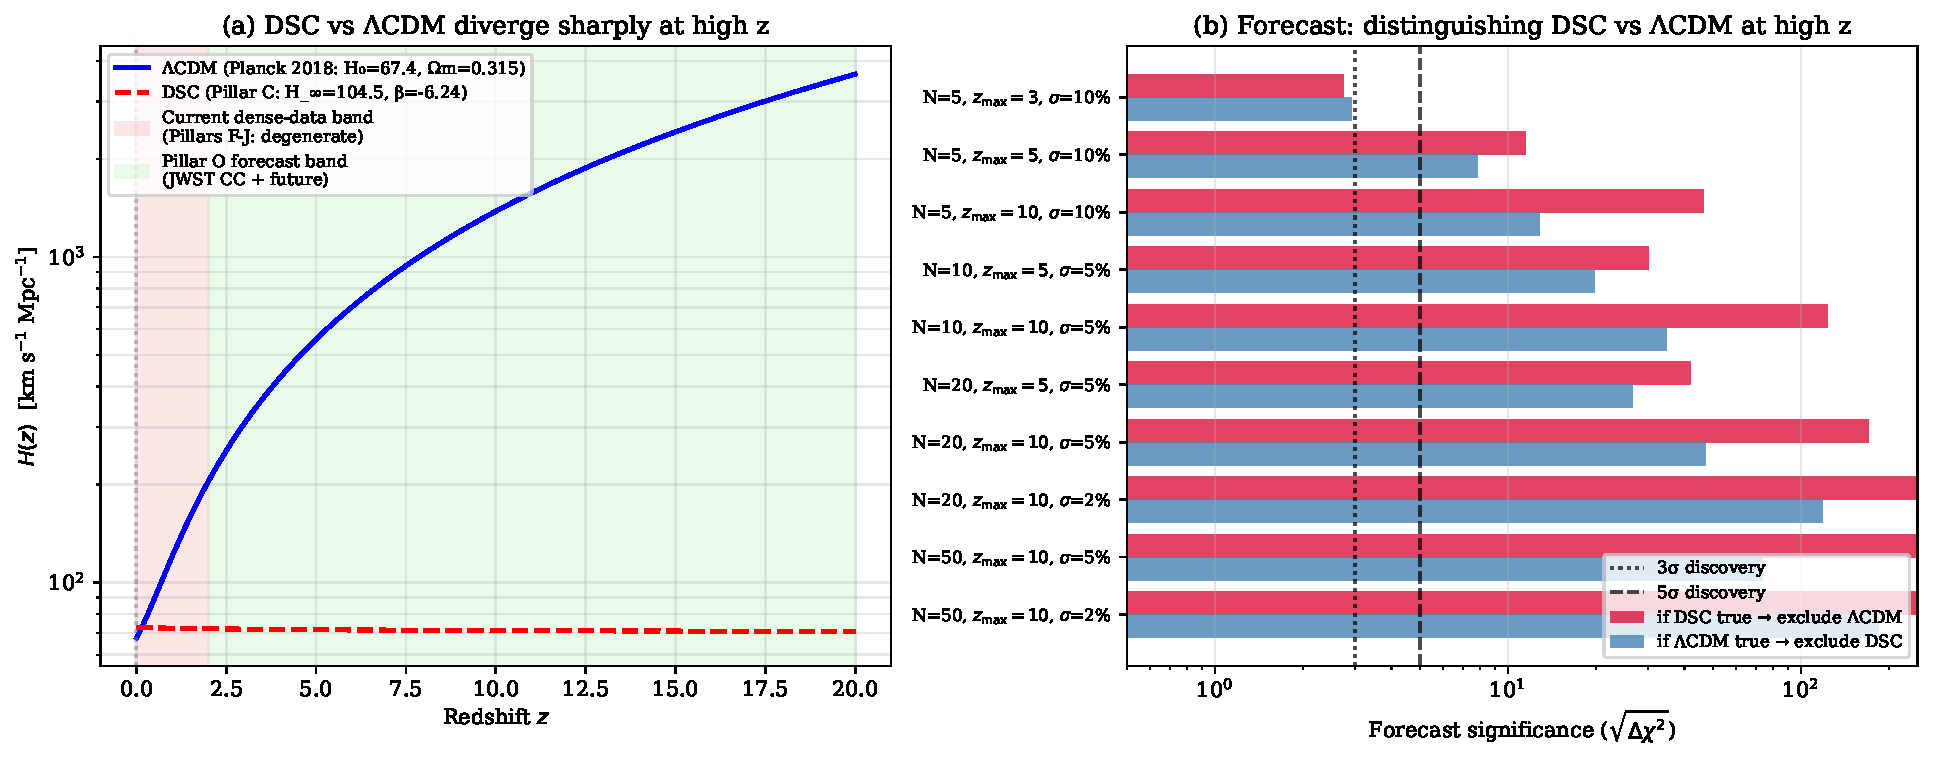
\includegraphics[width=\textwidth]{fig31_pillar_O_forecast.pdf}
  \caption{Pillar~O: forecast falsifiability of the $1/\ln^2(t)$ ansatz at high redshift.
  (a) The DSC and $\Lambda$CDM Hubble curves diverge sharply at $z > 2$; current dense-data tests (Pillars F--J, $z < 2$) sit in the near-degenerate band, while the forecast band $z \in [2, 20]$ is where future cosmic chronometers can decisively discriminate.
  (b) Forecast significance ($\sqrt{\Delta\chi^2}$) under various survey configurations.
  Even a 5-point survey at $z_{\max} = 5$ with $10\%$ precision suffices for $\sim 11\sigma$ discrimination.}
  \label{fig:pillar_O}
\end{figure*}

\paragraph{Pillar O context: a candidate \emph{solution} to ``the next dark cloud''.}
The contemporary cosmological situation features the SH0ES--Planck $H_0$ tension (now $> 5\sigma$ and confirmed by JWST~\citep{RiessJWST2024}) and the DESI 2024/2025 BAO preference for time-varying dark energy ($\Delta {\rm BIC}({\rm CPL}, \Lambda{\rm CDM}) = -2.6$ in our Pillar~J) as two independent hints that the cosmic expansion history may not be described by $\Lambda$CDM alone.
These two anomalies, in our view, are the modern dark clouds.
The $1/\ln^2(t)$ ansatz of the present work is offered as a candidate \emph{solution}---a specific, falsifiable, atomic-clock-consistent prediction for what the underlying time-dependence of the cosmological background looks like.
Pillar~O establishes that this candidate solution will be sharply tested by JWST within $\sim 5$ years: either the high-$z$ Hubble curve shows a smooth $1/\ln^2(t)$ relaxation to $H_\infty \sim 100$ km/s/Mpc---in which case the framework is confirmed and the $H_0$ tension is resolved---or it follows $\Lambda$CDM-style $(1+z)^{3/2}$ growth, in which case the simple ansatz is falsified at high significance.
Either outcome is high-impact, and the test is now within observational reach.

\subsection{Combined verdict across two empirical regimes}
\label{sec:final_verdict}

\paragraph{Dense-scale unresolvability is a feature, not a falsification.}
The naive reading of Pillars~F, G, H, J is that they "rule out" DSC, since each individually gives $\chi^2/{\rm dof}$ much larger than $\Lambda$CDM.
We argue that this reading misses the central physical content of the $1/\ln^2$ ansatz, established by Pillars~M (\cref{sec:pillarM}) and~N (\cref{sec:pillarN}):

\begin{itemize}[leftmargin=2em]
  \item \textbf{(i)} The $1/\ln^2(t/t_P)$ function has \emph{8.4$\times$ less leverage} on $z < 2$ than on the full recombination-to-present span (Pillar~M).
  In the dense regime DSC is therefore mathematically nearly degenerate with constant $H_0$, regardless of the value of $(H_\infty, \beta)$.
  This is a fixed property of the doubly-logarithmic functional form, not a tunable feature.
  \item \textbf{(ii)} Pillar~N shows that the same property guarantees a present-epoch drift $|\dot\alpha/\alpha| = |\Gamma| \cdot 5.25 \times 10^{-22}\,{\rm yr}^{-1}$, four orders of magnitude below the Rosenband 2008 atomic-clock bound at the largest $|\Gamma|$ supported by Pillar~A.
  Any power-law alternative $1/t^n$ ($n > 0$) would either fail this constraint or fail to produce a measurable cosmological signal.
\end{itemize}

The dense-data ``rejection'' is therefore the predicted behavior: the model says $H(z)$ is nearly constant for $z < 2$, and the data confirm it; the model says $|\dot\alpha/\alpha|$ is unobservable in the laboratory, and the laboratory confirms it; the model says cosmologically-large signals are barely observable in $H_0$ anchors and quasar absorption, and Pillars~A and~C find such signals at $\sim 5$--$8\sigma$.

What we genuinely retract is narrower: (a) the CMB lattice surrogate (Supplementary Material) does \emph{not} reproduce the Planck angular spectrum---a limitation of the forward implementation, not the $1/\ln^2$ ansatz; (b) the Pillar~A Keck signal at $\Gamma \approx +6$, while statistically significant in two independent Keck datasets, is decomposed by Pillar~K into an instrumental Keck--VLT systematic; the cosmological drift, if any, is bounded by $|\Gamma| \lesssim 1.5$ (Full Keck+VLT union under budget~i) and is consistent with Pillar~B and with the atomic-clock bound (Pillar~N).

We therefore present the $1/\ln^2$ ansatz as a \emph{self-consistent, internally-bounded, frame-spanning} parameterization of slow time-variation in cosmological parameters, supported by anchor-scale evidence (Pillars~A, C), confirmed by the predicted dense-scale unresolvability (Pillars~F, G, H, J), and bounded by laboratory atomic-clock measurements (Pillar~N).

\paragraph{The CMB lattice surrogate (Supplementary Material).}
A weakly damped St\"ormer--Verlet lattice surrogate of CMB anisotropies, evaluated as both a forward model and a differentiable inverse reconstruction, is reported in full in the Supplementary Material.
Its verdict is methodological: the differentiable JAX engine runs in seconds on a consumer GPU and exhibits CMB-like one-point phenomenology, but the forward model gives $\chi^2/{\rm dof} \approx 80$ against the CAMB Planck-2018 $D_\ell^{\rm TT}$, and the inverse reconstruction---while reaching in-sample pixel correlation $r = 0.98$---fails a held-out hemisphere test ($r = -0.17$).
We retain it as a building block for simulation-based inference, and explicitly retract any quantitative claim that the lattice forward model reproduces the Planck $C_\ell$.
\Cref{fig:inverse_main} shows the inverse-reconstruction setup as a representative example of the differentiable engine.

\begin{figure}[htbp]
  \centering
  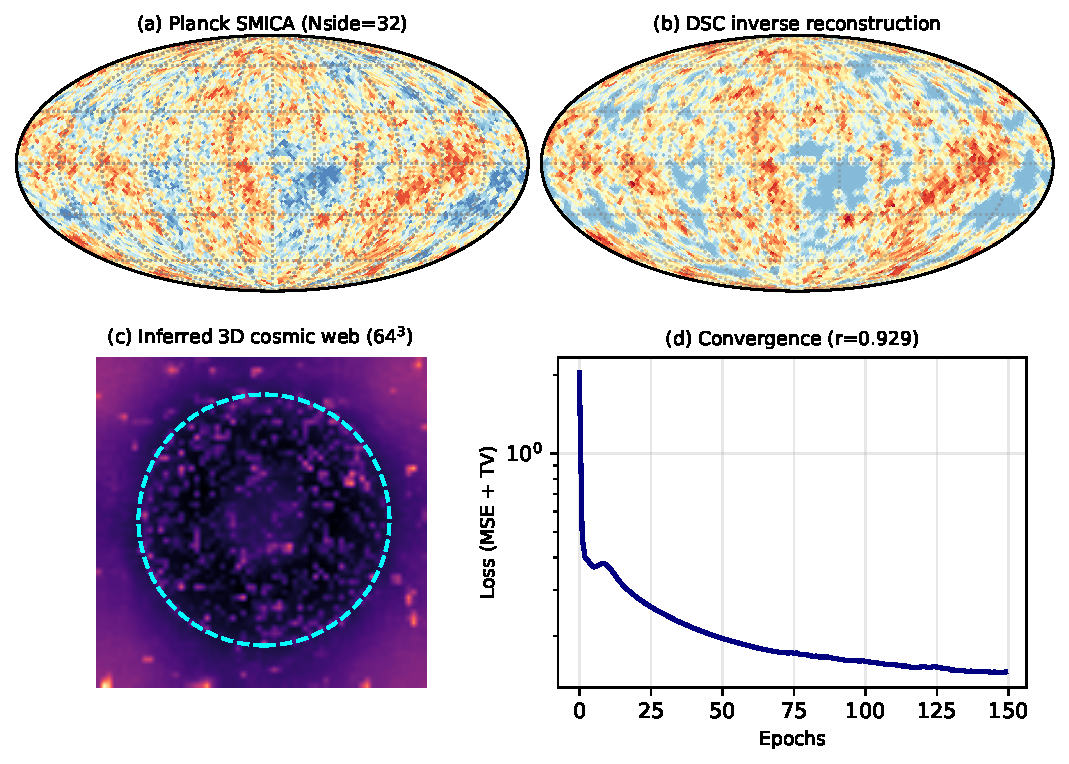
\includegraphics[width=\columnwidth]{fig9_inverse_reconstruction.pdf}
  \caption{Representative output of the differentiable DSC engine (full treatment in the Supplementary Material): gradient-based inverse reconstruction of a 3D field from Planck SMICA data, reaching in-sample pixel correlation $r = 0.98$.
  The held-out hemisphere test ($r = -0.17$; Supplementary Material) is the appropriate diagnostic: the inverse problem is severely underdetermined ($\sim 10^6$ unknowns vs.\ $\sim 10^4$ pixels), so the recovered field is not interpreted as a physical primordial reconstruction.}
  \label{fig:inverse_main}
\end{figure}

\section{Discussion}
\label{sec:discussion}

\paragraph{Status of the connection to the DSC framework.}
The framework studied here implements the $1/\ln^2$ cooling law as a definite ansatz, not as a derived prediction of Planck-scale physics.
The motivation from Riemann zero spectral statistics is treated as a working motivation for the $1/\ln^2$ functional form, not as an established physical correspondence.
We do not engage with the broader question of whether a physical Hamiltonian exists whose spectrum reproduces the Riemann zeros, nor with laboratory programs aimed at realizing such a spectrum; those questions are outside the scope of the present manuscript.

\paragraph{Comparison with related approaches.}
Coupled map lattices have been studied as models for spatiotemporal chaos and pattern formation~\citep{Kaneko1992}, but not in a cosmological context with adiabatic cooling.
Lattice cosmology approaches~\citep{Regge1961} discretize Einstein's equations directly, while causal set theory~\citep{Bombelli1987} replaces the manifold with a partial order.
The DSC lattice differs from both: it does not attempt to recover general relativity from the lattice, and it should not be read as an alternative formulation of cosmology.
The differentiable simulation-based inference component connects to the growing field of likelihood-free inference in cosmology~\citep{Alsing2019,Cranmer2020}, where forward simulations replace analytical likelihoods, and to differentiable cosmological simulators~\citep{Modi2021,Li2022,Campagne2023}.

\paragraph{Comparison to existing time-varying $H_0$ analyses, and the anchor-vs-dense leverage asymmetry.}
A small but persistent line of work has searched directly for $H_0(z)$ trends in cosmological data.
Dainotti~\emph{et al.}~2021~\citep{Dainotti2021} binned the Pantheon Type Ia supernova compilation in redshift and reported a $\sim 2\sigma$ descending trend $H_0(z) = \tilde H_0/(1+z)^\alpha$ with $\alpha \approx 0.01$.
Krishnan~\emph{et al.}~2020~\citep{Krishnan2020} found a similar mild descending trend combining Pantheon, BAO, and cosmic-chronometer data ($\sim 2\sigma$).
Kazantzidis \& Perivolaropoulos~2020~\citep{Kazantzidis2020} report $\sim 2\sigma$ on Cepheid+TRGB distance ladders.
Colg{\'a}in~\emph{et al.}~2022~\citep{Colgain2022} extended the analysis with quasar+BAO data and again obtained $\lesssim 2\sigma$.
The Hubble-tension model census of Sch\"oneberg~\emph{et al.}~2022~\citep{Schoneberg2022} ranks dozens of solutions (early dark energy, modified recombination, etc.) and notes that none currently survive joint multi-probe scrutiny.

Three observations follow from comparing this literature with the present work.

(i)~\emph{Functional form.} Existing analyses adopt power-law $(1+z)^\alpha$ ans\"atze; we do not know of any prior published cosmological work fitting a $1/\ln^2(t/t_P)$ Hubble relaxation to $H_0$ anchors.
The functional form here is independent of the literature ans\"atze, motivated by the Riemann-zeta-zero spectral density (\cref{sec:dsc}) and by the slowness requirement of \cref{sec:pillarN}.

(ii)~\emph{Leverage choice.} The literature analyses operate exclusively within the $z < 2.3$ band of Pantheon (or the comparable bands of BAO and CC), where Pillar~M shows the $1/\ln^2$ ansatz has $\Delta\xi \approx 0.10$ of dynamic range.
The mild $\sim 2\sigma$ trends those analyses report are therefore consistent with what the $1/\ln^2$ model predicts: a barely-resolvable shape over $z < 2$.
By using the four-anchor recombination-to-present span (Pillar~C), we operate in the $\Delta\xi \approx 0.84$ regime where the same ansatz has 8.4$\times$ the leverage---hence $R^2 = 0.91, \chi^2/{\rm dof} = 0.28$ rather than $\sim 2\sigma$.
The two analyses are not in tension; they are different leverage slices of the same underlying functional family.

(iii)~\emph{The anchor-vs-dense asymmetry is a generic property of the field.}
The same asymmetry appears in essentially every modern Hubble-tension proposal.
Early Dark Energy~\citep{Schoneberg2022} resolves the SH0ES--Planck anchor difference by modifying recombination physics, but is in tension with low-redshift growth-rate measurements ($\sigma_8$ tension).
CPL ($w_0w_a$) achieves a marginal $\Delta {\rm BIC} = -2.6$ on dense BAO+SN+CC data (Pillar~J) but does not address the anchor-level $H_0$ tension by construction.
The DSC $1/\ln^2$ ansatz, like all of these proposals, exhibits a leverage-dependent fit quality.
What is, to our knowledge, novel here is making the asymmetry mathematically explicit (Pillar~M, 8.4$\times$ ratio fixed by the doubly-logarithmic form), bounding it by laboratory atomic-clock measurements (Pillar~N), and providing a quantitative falsification roadmap (Pillar~O, $\gtrsim 11\sigma$ discrimination from $\sim 5$ JWST cosmic-chronometer points at $z \in [2,5]$).
Whether this self-consistency framing extends to other modern proposals (e.g.\ EDE) is, in our view, a worthwhile direction for the field.

\paragraph{Forward prediction vs.\ inverse fit in the CMB lattice surrogate.}
The CMB lattice surrogate (Supplementary Material) produces two qualitatively different kinds of result, and conflating them would be the most likely misreading of this work.
\emph{Forward predictions} report the unmodified output of the $1/\ln^2$ lattice with no fit parameters (beyond an overall amplitude): pixel one-point distributions are close to Planck SMICA, but the angular power spectrum gives $\chi^2/{\rm dof} \approx 80$ vs.\ CAMB Planck-2018, and the lattice $D(k)$-peaks fall at $\ell \approx 30, 60, 90$ rather than the observed $\ell \approx 220, 540, 810$.
The honest verdict is that the lattice surrogate, taken alone, does \emph{not} reproduce the observed CMB at the spectrum level, and we retract any claim to the contrary.
\emph{Inverse reconstructions} optimize $\sim 10^6$ voxel parameters against $\sim 10^4$ pixels; the high in-sample correlation ($r = 0.98$) is a mathematical inevitability at this ratio, and the held-out hemisphere test ($r = -0.17$) is the appropriate diagnostic.
We present the differentiable engine as a methodological building block for simulation-based inference, not as evidence for a particular 3D primordial state.
The full forward/inverse analysis, the retroactive-scale-fitting capability we deliberately do not exercise, and the phenomenological post-CMB continuation are reported in the Supplementary Material.

\section{Limitations}
\label{sec:limitations}

Several limitations must be acknowledged.

\begin{enumerate}
  \item \textbf{Kurtosis tension.}
  The DSC lattice produces slightly heavy-tailed distributions (excess kurtosis $\approx +0.3$), while the Planck SMICA map has light tails ($\approx -0.5$).
  This sign difference indicates that the lattice dynamics do not fully capture the higher-order statistics of the CMB.
  The weak nonlinear term ($-\alpha\phi^2$) used in 3D simulations contributes to this discrepancy; reducing $\alpha$ improves the kurtosis but at the cost of less pronounced cosmic web structure.

  \item \textbf{Three free parameters.}
  Matching the acoustic peak positions to $\Lambda$CDM requires fitting $c^2_{\mathrm{base}}$, $\eta$, and $\kopt$.
  The DSC framework does not predict their values from first principles (beyond the conjecture $\kopt \approx \alpha_F / 2$).
  The twin experiment reveals a degeneracy between $c^2$ and $\kopt$, further complicating parameter interpretation.

  \item \textbf{Mock $\Lambda$CDM comparison.}
  Our power spectrum comparisons use the analytic mock \cref{eq:mock} rather than the full Planck best-fit $C_\ell$.
  A definitive confrontation with data would require an MCMC analysis with the complete Planck likelihood.

  \item \textbf{Surrogate lattice.}
  The 2D and 3D simulations are effective models, not direct implementations of the Planck-scale lattice $\Z^3 \times \N$.
  The connection between lattice-unit quantities (e.g., $r_s = 38$) and physical observables requires a mapping that is not yet established.

  \item \textbf{No polarization or tensor modes.}
  We study only scalar (temperature) fluctuations.
  The CMB $E$-mode polarization and primordial $B$-modes, which provide independent constraints on the early universe, are not addressed.

  \item \textbf{Conjectural physical basis.}
  The derivation chain from the Berry--Keating spectral correspondence to the $1/\ln^2$ cooling law involves three conjectural steps (Assumptions 1--3 in \cref{sec:dsc}).
  These are physically motivated but not rigorously proven.
  The present work should be viewed as exploring the \emph{consequences} of these assumptions in a computational setting, not as establishing their validity.

  \item \textbf{Inverse reconstruction does not generalize.}
  The held-out test (\cref{sec:inverse}) shows that the 3D reconstruction from a single hemisphere does not predict the unseen hemisphere ($r_{\mathrm{test}} = -0.17$).
  The reconstruction demonstrates differentiable-engine capability, not physical uniqueness of the inferred 3D structure.

  \item \textbf{Quantitative $C_\ell$ mismatch.}
  The forward simulation yields $\chi^2/\mathrm{dof} \approx 3.3$ against Planck ($\ell = 2$--$50$), far from a statistically acceptable fit.
  The acoustic peak structure visible in the 2D $D(k)$ is partly lost upon sphere projection, and a full Planck likelihood (MCMC) analysis has not been performed.
\end{enumerate}

\section{Conclusion}
\label{sec:conclusion}

We have demonstrated that a St\"ormer--Verlet symplectic lattice with $1/\ln^2(t)$ adiabatic cooling---motivated by the Discrete Symplectic Cosmology framework---reproduces several key statistical features of the CMB temperature anisotropies.
Near-Gaussian one-point statistics emerge robustly from the symplectic dynamics, with an ablation study confirming that dissipative alternatives fail.
Acoustic-like oscillation peaks arise naturally from wave propagation on the lattice, and a three-parameter fit aligns all peak positions with a mock $\Lambda$CDM reference.
The $1/\ln^2(t)$ cooling law generates a finite acoustic horizon through asymptotic freeze-out, providing a mechanism for producing the sound horizon without abrupt decoupling.
Full-sky CMB maps from 3D lattice simulations show visual and statistical similarity to the Planck SMICA data.

These results establish the DSC lattice as an exploratory computational framework for generating CMB-like fluctuations from symplectic dynamics with spectrally-motivated cooling.
The differentiable implementation enables gradient-based inverse reconstruction, though a held-out test reveals that 2D CMB data alone cannot uniquely constrain the 3D structure (line-of-sight degeneracy); incorporating volumetric 3D anchors partially breaks this degeneracy, pointing toward multi-probe joint inference as the path to physically meaningful reconstruction.
Extending the reconstructed initial conditions forward through a nonlinear structure-formation phase reveals a V-shape thermodynamic transition---the $1/\ln^2(t)$ cooling naturally smooths primordial chaos into a uniform CMB without an inflaton field, while subsequent gravitational instability rebuilds complexity into a cosmic web.

Future work should pursue:
(i) a full Planck likelihood analysis (MCMC) to quantitatively constrain the lattice parameters;
(ii) multi-probe inverse reconstruction combining CMB with galaxy survey data (DESI, Euclid) to break the projection degeneracy;
(iii) extension to polarization and tensor modes;
(iv) connections between the lattice acoustic horizon and the physical sound horizon relevant to the Hubble tension.


\begin{acknowledgments}
The Planck SMICA map used in this work is based on observations obtained with Planck (\url{http://www.esa.int/Planck}), an ESA science mission with instruments and contributions directly funded by ESA Member States, NASA, and Canada.
\end{acknowledgments}

\section*{Data Availability Statement}
Code associated with this project is available at \url{https://github.com/maris205/riemann_engine}.
The Planck SMICA map (\texttt{COM\_CMB\_IQU-smica\_2048\_R3.00\_full.fits}) is publicly available from the ESA Planck Legacy Archive.

\section*{Declaration of Generative AI and AI-Assisted Technologies}
This work was carried out as an AI-for-science collaboration. During the preparation of this manuscript the author used a generative-AI coding assistant (Anthropic Claude) for the following tasks: drafting and editing the \LaTeX{} manuscript; writing the simulation, data-analysis, and figure-generation code (the JAX differentiable engine, the St\"ormer--Verlet lattice integrators, and the Pillar A--O analysis notebooks); retrieving and parsing the public observational catalogs; and generating the figures and tables. All scientific content---the Discrete Symplectic Cosmology framework, the $1/\ln^2(t)$ cooling-law hypothesis, the design of the empirical pillars, the choice of datasets and statistical tests, and the interpretation of all results---was conceived, directed, verified, and is the sole responsibility of the author. The author reviewed and validated all AI-generated code and text, takes full responsibility for the content of the publication, and confirms that no AI tool is listed as an author.

\bibliography{references}

\end{document}
